\newpage

\chapter{Techno-Economic Analysis}

\section{Budget}

\begin{figure}[H]
	\centering
	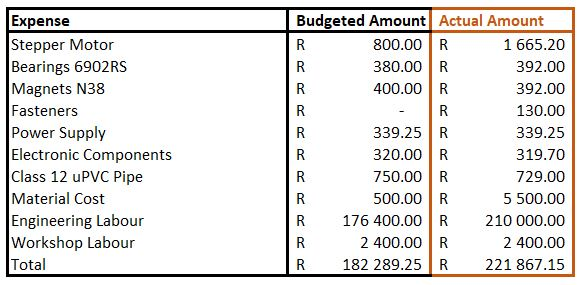
\includegraphics[width=\linewidth]{Budget.jpg}
	\label{fig:budget}
\end{figure}

\begin{figure}[H]
	\centering
	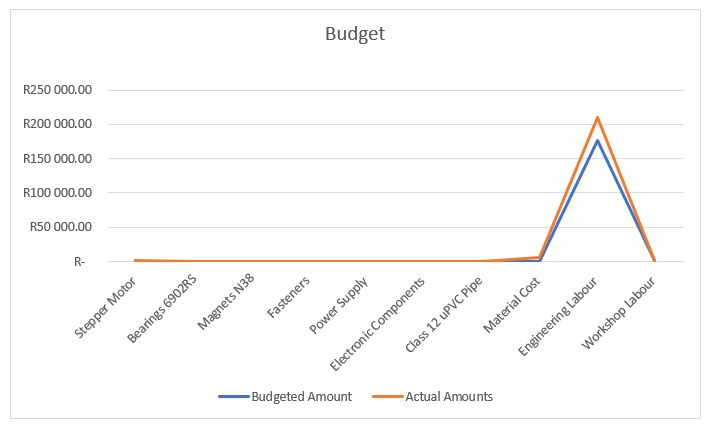
\includegraphics[width=\linewidth]{BudgetGraph.jpg}
	\label{fig:budgetgraph}
\end{figure}

\section{Time Management}

\begin{figure}[H]
	\centering
	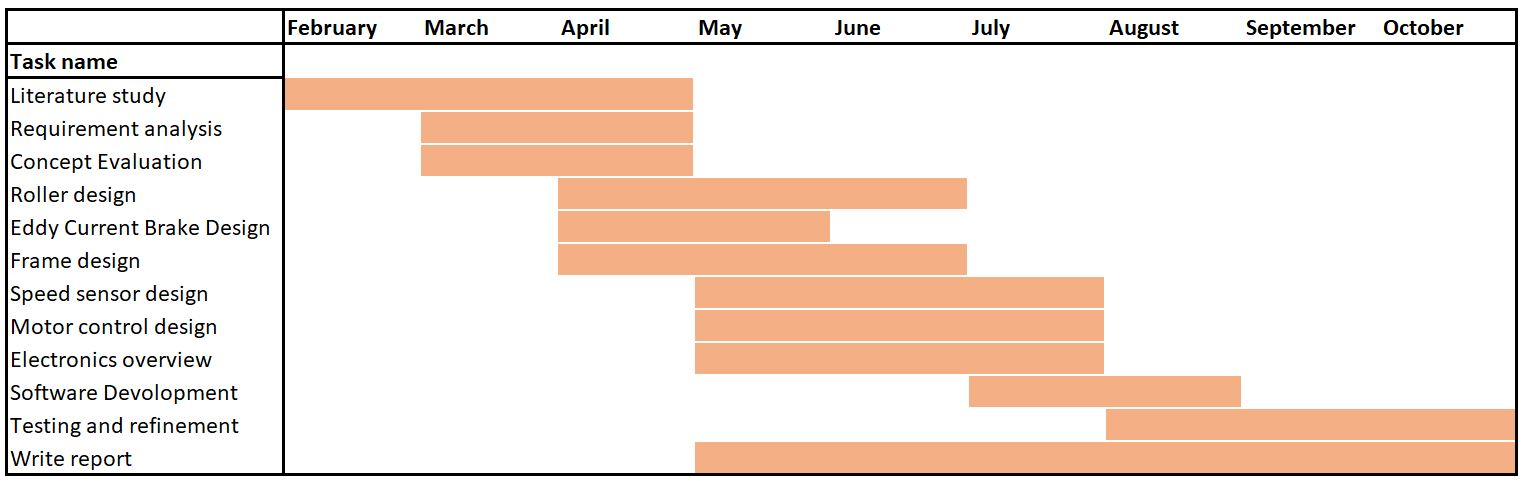
\includegraphics[width=\linewidth]{Gantt.jpg}
	\caption{Planned Schedule Gantt Chart}
	\label{fig:gantt}
\end{figure}

\begin{figure}[H]
	\centering
	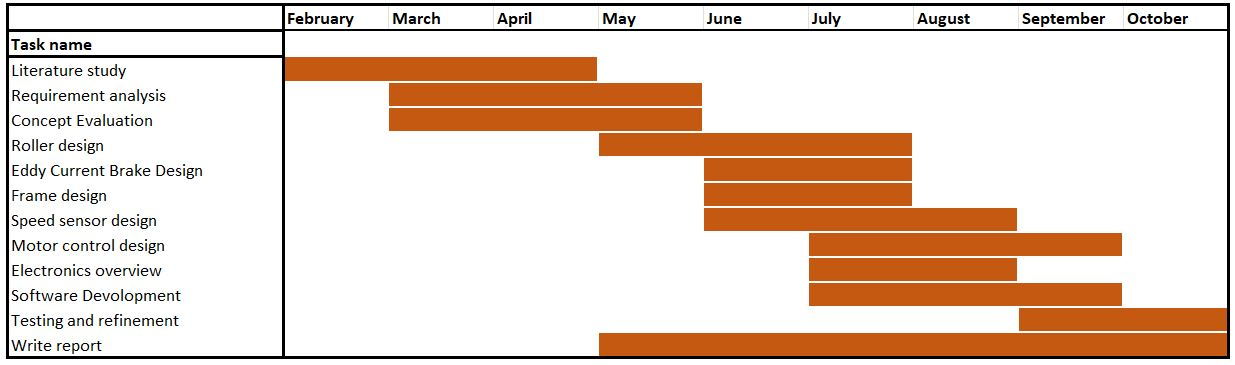
\includegraphics[width=\linewidth]{GanttActual.jpg}
	\caption{Actual Project Gantt Chart}
	\label{fig:ganttact}
\end{figure}

\section{Technical Impact}

The contribution of open-source code with projects like the one in this report enable more projects to be developed in similar fields in the future. Although similar projects developing smart trainers are available on the internet, there are no examples of accessible code that implements the \ac{ftms} Bluetooth protocol for communicating with the Zwift application.

\section{Return on Investment}

Design research projects such as this can give valuable insight into the workings of existing market products that are not accessible to some consumers due to various different factors. Due to no real goal of monetization, it is difficult to qualitatively measure the return that is gained from this project. The biggest value proposition that the project adds is the publicity from making the researched knowledge and information available for further development and expansion in the future. This leads to a net gain for the pool of available knowledge in this field.

\section{Potential for Commercialization}

The market for smart trainers is very competitive, with large companies like Garmin and Huawai having subsidiaries selling products in this space. The intention of the trainer development in this project was never aimed at delivering a commercially viable model, but rather at demonstrating the development process utilising the software developed in this project. This will allow other developers and consumers around the world to apply the reported knowledge to their own respective projects.